\chapter[RMN 2D]{Expériences à deux dimensions}

Une séquence impulsionnelle dont le but est la production d'un spectre de RMN 2D
n'est pas plus difficile à analyser qu'une séquence 1D.
Elle est en effet constituée d'impulsions de radio-fréquence et
de gradient de champ statique séparées par des délais
ou des périodes d'acquisition du signal.
L'acquis théorique des chapitres précédents trouve naturellement
ici un nouveau domaine d'application.

\section{Généralités}
\label{sec:2d:gen}
L'utilisation de la plus fréquente de la RMN 2D est
la recherche de paires de noyaux couplés.
Il est alors question de spectres 2D de corrélation des déplacements chimiques.
Cette expression indique que le déplacement chimique d'un noyau
est corrélé à celui d'un d'autre noyau si ces deux noyaux sont couplés ensemble.
L'acronyme COSY a été formée à partir de l'expression "COrrelation SpectroscopY".
L'expérience historique relatée en 1971 a été suivie de très nombreux
développements et d'autres séquences impulsionnelles dédiées à la spectroscopie de 
corrélation ont vu le jour et reçu diverses appellations.

Le grand intérêt de la RMN 2D est de concentrer sur un seul spectre l'information
relative à toutes les paires de noyaux, pour un type de couplage donné.
On distingue en effet les spectres 2D homonucléaires (\prot -- \prot, comme les spectres COSY et NOESY)
des spectres 2D hétéronucléaires (\prot -- \carb par exemple, comme le spectre HSQC).
La recherche de paires de noyaux couplés est une étape essentielle à
l'interprétation des spectres de molécules complexes.
En effet, l'existence
d'un couplage scalaire indique que les noyaux concernés sont séparés par un
petit nombre de liaisons chimiques ; elle fournit donc une information
sur la connectivité des atomes d'une molécule, c'est-à-dire sur sa formule
développée plane.
De plus, un couplage dipolaire est une source de relaxation croisée
et révèle donc une proximité spatiale entre les noyaux.
Un spectre NOESY permet ainsi de préciser la configuration d'une molécule,
c'est-à-dire sa structure tridimensionnelle.

En plus de la corrélation des déplacements chimiques,
une autre famille d'expériences de RMN 2D produit des spectres
dits "de séparation des interactions".
Dans cette catégorie, un spectre $J$-résolu fournit une vision
séparée des déplacements chimiques
et des motifs de couplage scalaire. 
Cette expérience facilite la mesure
de ces constantes et vient compléter les informations conformationnelles apportées
par l'expérience NOESY, elle permet
de plus une lecture simplifiée des déplacements chimiques

Pour tenter de réduire la difficulté d'apprentissage 
des concepts spécifiques à la RMN 2D (ou nD...) la séquence COSY
"à un seul noyau" sera d'abord traitée.
Il n'y a aucun intérêt à utiliser la séquence COSY sur des systèmes à un spin
puisque le but de la séquence COSY
est de révéler les couplages entre deux noyaux.
Toutefois, l'analyse de la séquence COSY sur un tel système
est commode pour introduire le concept de modulation et montrer
comment le problème central de la détermination du signe des fréquences dans
les deux dimensions a été résolu.
Les résultats généraux obtenus à partir de cet exemple
faciliteront l'étude des autres séquences.
La COSY "à un noyau" ne faisant pas intervenir de système de spins couplés,
la description vectorielle de l'évolution de l'aimantation nucléaire est suffisante.
Cela réduit au minimum l'aspect calculatoire, souvent dissuasif, des explications
relatives à la compréhension de la RMN 2D.

\section{La COSY "à un noyau"}
\label{sec:2d:cosy1noyau}
\subsection{Séquence}
\label{sec:2d:cosy1noyau:seq}
La séquence de base, figure \ref{fig:cosydebase}, est constituée d'un délai de relaxation,
d'une impulsion d'excitation, d'un délai d'évolution de durée nommé $t_1$, 
d'une impulsion dite "de transfert" et d'une période
d'acquisition où le signal est mesuré aux instants $t_2$.
Cette séquence n'est autre qu'une séquence 1D un peu particulière.
L'expérience n'acquiert l'appellation 2D que si elle est réalisée pour plusieurs valeurs
de $t_1$.
Les angles de nutation des deux impulsions seront considérés comme égaux à $\pi/2$.
Le signal enregistré est une fonction de $t_2$  mais aussi du temps 
$t_1$ et des phase $\phi_1$ et $\phi_2$ des impulsions.
En fait, seule la phase relative des impulsions est significative puisque leur augmentation
simultanée de $\pi/2$ produit une multiplication du signal par $i$
qui peut être compensée en augmentant la phase du récepteur de $\pi/2$.
Le système étudié est un ensemble de noyaux identiques notés
$I$ et caractérisés par leur offset $\omsi$
et leurs temps de relaxation $T_{1I}$ et $T_{2I}$.
L'effet des inhomogénéités de $\bzeros$ ne sera pas pris en compte dans un premier temps.

\begin{figure}[hbt]
\begin{center}
\begin{pspicture}(0,0)(7,3)
% sequence I
\rput(1,1.5){
\psline(0,0)(6,0)
\rput(-0.5,0){RF($I$)}
\psline[linewidth=2mm]{-}(1,0)(1,1)
\rput(1,1.2){$\phi_1$}
\psline[linewidth=2mm]{-}(4,0)(4,1)
\rput(4,1.2){$\phi_2$}
\rput(4.1,0){
\pscurve(0,0.5)(0.5,0.25)(1.5,0)
\pscurve(0,-0.5)(0.5,-0.25)(1.5,0)
\psline(0,0.5)(0,-0.5)
}
\rput(5,0.5){$\phi_R$}
}
% time marks
\rput(1,0.5){
\psline{->}(0,0)(6,0)
\rput(6.2,0){$t$}
\psline[linewidth=0.25mm,linestyle=dashed]{-}(0.9,0.8)(0.9,-0.2)
\rput(0.8,-0.4){A}
\psline[linewidth=0.25mm,linestyle=dashed]{-}(1.1,0.8)(1.1,-0.2)
\rput(1.2,-0.4){B}
\rput(2.5,0.5){$t_1$}
\psline[linewidth=0.25mm,linestyle=dashed]{-}(3.9,0.8)(3.9,-0.2)
\rput(3.8,-0.4){C}
\psline[linewidth=0.25mm,linestyle=dashed]{-}(4.1,0.8)(4.1,-0.2)
\rput(4.2,-0.4){D}
\psline[linewidth=0.25mm,linestyle=dashed]{-}(5,0.8)(5,-0.2)
\rput(5.3,0.5){$t_2$}
}
\end{pspicture}
\caption{\label{fig:cosydebase}
Séquence COSY}
\end{center}
\end{figure}

\subsection{Modulation d'amplitude, méthode de States}
\label{sec:2d:cosy1noyau:amp}
L'aimantation initiale
\begin{equation}
\aimvec(t_A) = \aimzeros\coo{0}{0}{1}
\end{equation}
devient
\begin{equation}
\aimvec(t_B) = \aimzeros\coo{0}{-1}{0} \qsiq \phi_1 = 0 \qetq
\aimvec(t_B) = \aimzeros\coo{1}{0}{0} \qsiq \phi_1 = \pi/2
\end{equation}
après la première impulsion.
Après le délai de durée $t_1$, l'aimantation devient
\begin{eqnarray}
\label{eqn:rmn2d1:tcs}
\aimvec(t_C) & = & \aimzeros\coo{\sin(\omsi t_1)}{-\cos(\omsi t_1)}{0} \qsiq \phi_1 = 0 \\
\label{eqn:rmn2d1:tcc}
\aimvec(t_C) & = & \aimzeros\coo{\cos(\omsi t_1)}{\sin(\omsi t_1)}{0} \qsiq \phi_1 = \pi/2
\end{eqnarray}
en considérant que ni la relaxation transversale ni la relaxation longitudinale
ne sont intervenus pendant $t_1$.
En réalité, leur action se traduit par le facteur d'amortissement de l'aimantation transversale
$r_{2I}(t_1) = \exp(-t_1/T_{2I})$ et le facteur de "repousse" de l'aimantation longitudinale
$r_{1I}(t_1) = 1 - \exp(-t_1/T_{1I})$ (équations \ref{eqn:relaxlong} et \ref{eqn:relaxtrans}),
si bien que les équations \ref{eqn:rmn2d1:tcs} et \ref{eqn:rmn2d1:tcc} deviennent :
\begin{eqnarray}
\aimvec(t_C) & = & 
\aimzeros\coo{\sin(\omsi t_1) r_{2I}(t_1)}{-\cos(\omsi t_1) r_{2I}(t_1)}{r_{1I}(t_1)}
\qsiq \phi_1 = 0 \\
\aimvec(t_C) & = & 
\aimzeros\coo{\cos(\omsi t_1) r_{2I}(t_1)}{\sin(\omsi t_1) r_{2I}(t_1)}{r_{1I}(t_1)} 
\qsiq \phi_1 = \pi/2
\end{eqnarray}
La seconde impulsion, de phase 0 ou $\pi$, préserve la composante sur l'axe $OX$ de
l'aimantation transversale et transfère l'autre sur l'axe $OZ$. 
La composante initialement présente sur $OZ$ est basculée dans le plan 
transversal sur l'axe $OY$.
Avec $\phi_2$ = 0,
\begin{eqnarray}
\label{eqn:rmn2d1aimxx}
\aimvec(t_D) & = &
\aimzeros\coo{\sin(\omsi t_1) r_{2I}(t_1)}{-r_{1I}(t_1)}{-\cos(\omsi t_1) r_{2I}(t_1)}
\qsiq \phi_1 = 0 \\
\label{eqn:rmn2d1aimyx}
\aimvec(t_D) & = & 
\aimzeros\coo{\cos(\omsi t_1) r_{2I}(t_1)}{-r_{1I}(t_1)}{\sin(\omsi t_1) r_{2I}(t_1)}
\qsiq \phi_1 = \pi/2
\end{eqnarray}
Dans les deux cas, la composante de l'aimantation sur l'axe $OX$ immédiatement avant le début
de l'acquisition du signal est identique à celle obtenue par application
d'une unique impulsion de phase $y$, à ceci près que l'\emph{amplitude}
est en ici modulée par un facteur qui dépend du produit $\omsi t_1$.
La modulation est dite "en sinus" quand les axes de rotation associés aux deux impulsions
sont colinéaires et "en cosinus" quand ils sont orthogonaux.

L'aimantation présente sur l'axe $OX$ donne lieu aux signaux
\begin{eqnarray}
s_S(t_1, t_2) & = & s_0 \sin(\omsi t_1) r_{2I}(t_1) \times \exp(i \omsi t_2 ) r_{2I}(t_2) \\
s_C(t_1, t_2) & = & s_0 \cos(\omsi t_1) r_{2I}(t_1) \times \exp(i \omsi t_2 ) r_{2I}(t_2)
\end{eqnarray}
où les indices $S$ et $C$ font référence aux deux types de modulation d'amplitude et $s_0$
est l'intensité du {\FID} obtenu par une seule impulsion de phase $\pi/2$.
La quantité $s_0$ est un nombre réel, ce qui sous-entend que le détecteur n'introduit pas
de déphasage du signal. Le facteur multiplicatif $s_0$ sera considéré par la suite 
comme égal à 1, sans perte de généralité pour l'exposé.
La partie réelle des signaux temporels est représentée sur la partie gauche
de la figure \ref{fig:modulampl}.
La TF de ces signaux, considérés comme des fonctions de la variable 
temporelle d'acquisition $t_2$ donne
\begin{eqnarray}
f_S(t_1, \Omega_2) & = & \sin(\omsi t_1) r_{2I}(t_1)
\times (A_I(\Omega_2-\omsi) + iD_I(\Omega_2-\omsi)) \\
f_C(t_1, \Omega_2) & = & \cos(\omsi t_1) r_{2I}(t_1)
\times (A_I(\Omega_2-\omsi) + iD_I(\Omega_2-\omsi))
\end{eqnarray}
où $A_I(\Omega_2)$ et $D_I(\Omega_2)$ sont les fonctions lorentziennes en absorption
et en dispersion centrées autour de la fréquence nulle.
La temps d'acquisition étant nommé $t_2$, la variable fréquentielle
associée a été nommée $\Omega_2$.
\begin{figure}[hbt]
\begin{center}
\begin{pspicture}(-0.5,-1)(13.5,7)
\psset{unit=5mm,labelsep=3pt}
\rput(0,0){
\rput(0,0){
\multido{\i=0+1}{24}
{
  \FPeval{yy}{\i/24*5}
  \FPeval{absc}{\i*0.1}
  \FPeval{ordo}{\i*0.5}
  \FPupn{facta}{yy 0.3 mul 2 mul \FPpi{} mul sin}
  \FPupn{factb}{yy 4 div neg exp}
  \FPupn{factc}{0.8}
  \FPupn{fact}{facta factb mul factc mul}
  \rput(\absc,\ordo)
  {
    \psplot[algebraic,plotpoints=200]{0}{5}{\fact*cos(x*2*\FPpi)*(\FPe^(-x/4))}
  }
}
\rput(-1,0){\psline{->}(0,0)(2.4,12)\uput[70](2.4,12){$t_1$}}
\rput(0,-1){\psline{->}(0,0)(5,0)\uput[-70](5,0){$t_2$}}
\rput(2.5,-2){$s_S(t_1,t_2)$}
}
\rput(6,0){
\multido{\i=0+1}{24}
{
  \FPeval{yy}{\i/24*5}
  \FPeval{absc}{\i*0.1}
  \FPeval{ordo}{\i*0.5}
  \FPupn{facta}{yy 0.3 mul 2 mul \FPpi{} mul cos}
  \FPupn{factb}{yy 4 div neg exp}
  \FPupn{factc}{0.8}
  \FPupn{fact}{facta factb mul factc mul}
  \rput(\absc,\ordo)
  {
    \psplot[algebraic,plotpoints=200]{0}{5}{\fact*cos(x*2*\FPpi)*(\FPe^(-x/4))}
  }
}
\rput(0,-1){\psline{->}(0,0)(5,0)\uput[-70](5,0){$t_2$}}
\rput(2.5,-2){$s_C(t_1,t_2)$}
}
}
%
\rput(14,0){
\rput(0,0){
\multido{\i=0+1}{24}
{
  \FPeval{yy}{\i/24*5}
  \FPeval{absc}{\i*0.1}
  \FPeval{ordo}{\i*0.5}
  \FPupn{facta}{yy 0.3 mul 2 mul \FPpi{} mul sin}
  \FPupn{factb}{yy 4 div neg exp}
  \FPupn{factc}{0.9}
  \FPupn{fact}{facta factb mul factc mul}
  \rput(\absc,\ordo)
  {
    \psplot[algebraic,plotpoints=200]{0}{5}{\fact/(1+((x-2.5)/0.2)^2)}
  }
}
\rput(-1,0){\psline{->}(0,0)(2.4,12)\uput[70](2.4,12){$t_1$}}
\rput(0,-1){\psline{<-}(0,0)(5,0)\uput[-110](0,0){$\Omega_2$}}
\rput(2.5,-2){$f_S(t_1,\Omega_2)$}
}
\rput(6,0){
\multido{\i=0+1}{24}
{
  \FPeval{yy}{\i/24*5}
  \FPeval{absc}{\i*0.1}
  \FPeval{ordo}{\i*0.5}
  \FPupn{facta}{yy 0.3 mul 2 mul \FPpi{} mul cos}
  \FPupn{factb}{yy 4 div neg exp}
  \FPupn{factc}{0.9}
  \FPupn{fact}{facta factb mul factc mul}
  \rput(\absc,\ordo)
  {
    \psplot[algebraic,plotpoints=200]{0}{5}{\fact/(1+((x-2.5)/0.2)^2)}
  }
}
\rput(0,-1){\psline{<-}(0,0)(5,0)\uput[-110](0,0){$\Omega_2$}}
\rput(2.5,-2){$f_C(t_1,\Omega_2)$}
}
}
\end{pspicture}
\caption{\label{fig:modulampl}
Signaux temporels 2D modulés en amplitude (à gauche) et leur TF (à droite)}
\end{center}
\end{figure}
La partie réelle des spectres, dont les intensités sont
modulées en sinus et en cosinus (voir la partie droite de la figure \ref{fig:modulampl})
peuvent être combinées pour donner un signal complexe virtuel (c'est-à-dire fabriqué
sans avoir été enregistré physiquement) $f(t_1, \Omega_2)$
dont l'intérêt apparaîtra bientôt.
\begin{eqnarray}
f(t_1, \Omega_2) & = & \reel(f_S(t_1, \Omega_2)) + i\reel(f_C(t_1, \Omega_2)) \\
\label{eq:rmn2d1:virtuel}
                 & = & i \exp(-i \omsi t_1) r_{2I}(t_1) \times A_I(\Omega_2-\omsi)
\end{eqnarray}
Ainsi $f(t_1, \Omega_2)$, considéré pour chaque valeur de $\Omega_2$,
varie en fonction de $t_1$ comme un {\FID} ordinaire.
Avec la méthode choisie pour la construction de la fonction $f$,
c'est la pulsation $-\omsi$ qui intervient pendant $t_1$
puisque $\sin x + i\cos x = i(\cos x - i \sin x) = i\exp(-ix)$.
De la même manière qu'un {\FID} est enregistré à partir de $t_2 = 0$ par intervalles
$\delta t_2 = 1/\Delta F_2$ pour
disposer d'une fenêtre spectrale de largeur $\Delta F_2$,
il suffit de faire varier $t_1$ à partir de 0 
par pas $\delta t_1 = 1/\Delta F_1$ pour déterminer
la fréquence d'évolution de l'aimantation pendant $t_1$
à l'intérieur d'une fenêtre spectrale de largeur $\Delta F_1$.
La TF de toutes les fonctions $S(t_1, \Omega_2)$, chacune correspondant 
à une valeur particulière de $\Omega_2$ et étant donc considérée comme une fonction
de la variable temporelle $t_1$, fournit
\begin{equation}
S(\Omega_1, \Omega_2) = i \times (A_I(\Omega_1+\omsi) + iD_I(\Omega_1+\omsi)) 
\times A_I(\Omega_2-\omsi)
\end{equation}
Une correction de phase de $\pi/2$ (une multiplication par $-i$) et la conservation de la seule
partie réelle conduit à
\begin{equation}
S(\Omega_1, \Omega_2) = A_I(\Omega_1+\omsi)  \times A_I(\Omega_2-\omsi)
\end{equation}
qui correspond à une raie élémentaire en absorption pure d'un spectre de RMN 2D,
et dont le maximum se trouve à $(\Omega_1, \Omega_2) = (-\omsi, \omsi)$.
Dans la pratique,le spectre 2D
est représenté en fonction de $-\Omega_1$ (sur un axe vertical dirigé de haut en bas)
et de $\Omega_2$ (sur un axe horizontal dirigé, comme en RMN 1D, de droite à gauche)
de sorte que l'évolution de l'aimantation
d'un même noyau pendant $t_1$ et $t_2$ se traduit par un pic situé sur la diagonale principale
du spectre, orientée du haut à droite vers le bas à gauche
dans le sens des déplacements chimiques croissants.
Les axes verticaux et horizontaux sont respectivement désignés sous le noms d'axes $F_1$ et $F_2$.
La figure \ref{fig:raies2D} fournit une représentation graphique
des formes de raies usuelles en RMN 2D.

\renewcommand{\baselinestretch}{1}
\normalsize
\begin{figure}[hbt]
\begin{center}

\begin{tabular}{llll}
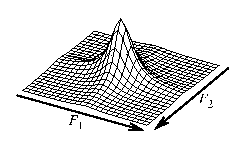
\includegraphics[scale=0.9]{ContSurf/surf1.eps} & 

\includegraphics[scale=0.9]{ContSurf/surf2.eps} & 

\includegraphics[scale=0.9]{ContSurf/surf3.eps} & 

\includegraphics[scale=0.9]{ContSurf/surf4.eps} \\
\rule[0mm]{0mm}{2mm} \\
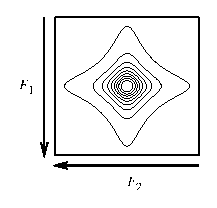
\includegraphics[scale=0.9]{ContSurf/cont1.eps} & 
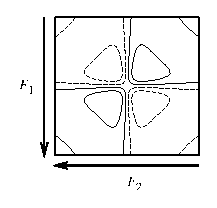
\includegraphics[scale=0.9]{ContSurf/cont2.eps} & 
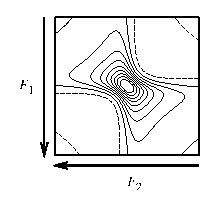
\includegraphics[scale=0.9]{ContSurf/cont3.eps} & 
\includegraphics[scale=0.9]{ContSurf/cont4.eps} \\
\myc{\raisebox{-0.5ex}[0pt]{Double}} &
\myc{\raisebox{-0.5ex}[0pt]{Double}} &
\myc{\raisebox{-0.5ex}[0pt]{Phase}} \\
\myc{Absorption} & 
\myc{Dispersion} & 
\myc{Twist} & 
\myc{\raisebox{1.25ex}[0pt]{Magnitude}}

\end{tabular}
\caption{\label{fig:raies2D}Formes de raies en RMN 2D}
\end{center}
\end{figure}
\renewcommand{\baselinestretch}{1.5}
\normalsize
Le cas particulier qui a été détaillé dans les paragraphes précédents est celui où 
le noyau dont l'aimantation évolue pendant $t_1$ ($I$) est le même que celui
dont l'aimantation évolue pendant $t_2$.
Dans le cas général, il faut considérer que l'aimantation d'un noyau $S$,
qui évolue pendant $t_1$, est transférée sur un noyau $I$ avant la détection
du signal créé par ce dernier.
Alors, les signaux enregistrés dépendent de $t_1$ au travers de facteurs
$\sin(\omss t_1)$ ou $\cos(\omss t_1)$ multipliés par un facteur d'amortissement
$r_{2S}=\exp(-t_1/T_{2S})$ où $\omss$ et $T_{2S}$ caractérisent le noyau S :
\begin{eqnarray}
s_S(t_1, t_2) & = & \sin(\omss t_1) r_{2S}(t_1) \times \exp(i \omsi t_2 ) r_{2I}(t_2) \\
s_C(t_1, t_2) & = & \cos(\omss t_1) r_{2S}(t_1) \times \exp(i \omsi t_2 ) r_{2I}(t_2)
\end{eqnarray}
L'expérience COSY, effectuée sur un système à un spin, ne peut pas donner
lieu à un transfert d'aimantation, ce qui conduit à identifier $S$ avec $I$.
D'une manière encore plus générale, la fréquence d'évolution pendant $t_1$
peut n'être ni $\omsi$ ni $\omss$, mais une autre comme $\omsi + \omss$, fréquence
d'évolution des états à double quanta dans un spectre INADEQUATE
ou encore $\pi J$ dans un spectre $J$-résolu.

Ce qui vient d'être décrit passe sous silence les signaux issus des composantes de
l'aimantation sur l'axe $OY$ décrites dans les équations
\ref{eqn:rmn2d1aimxx} et \ref{eqn:rmn2d1aimyx}.
Leur évolution en fonction de $t_1$ ne comporte aucune partie oscillante et sa TF selon $t_1$
produit un pic centré autour de la fréquence $\Omega_1$ nulle.
En effet, dans le facteur $1-\exp(-t_1/T_{1I})$, le terme 1 conduit à un
spectre nul partout sauf
pour $\Omega_1 = 0$ et le terme $-\exp(-t_1/T_{1I})$ conduit à une raie lorentzienne
centrée sur $\Omega_1 = 0$.
Si $t_1$ est suffisamment grand par rapport à $T_{1I}$ pour que $r_{1I}$ soit
significativement non nul, alors des pics indésirables sont visibles sur l'axe 
$F_1$ du spectre.
Ces pics axiaux sont éliminés par action du programme de phase de la séquence.
Si $\phi_2 = \pi$ au lieu de $0$, alors, à l'instant $t=t_D$
la composante de l'aimantation sur l'axe $OX$ est inchangée et celle sur $OY$
est inversée. 
Le signal indésirable est donc éliminé par addition des {\FID} produits
avec $\phi_2 = 0$ et $\phi_2 = \pi$.
Le nombre de scans minimum par valeur de $t_1$ nécessaire pour obtenir un spectre 2D
dépourvu de pic axiaux est donc de 4, 2 pour chaque type de modulation.

L'ensemble de la procédure d'acquisition et de traitement qui vient d'être décrite
fournit à la fois des pics en absorption pure et permet de déterminer le signe
de la fréquence d'évolution de l'aimantation pendant $t_1$.
Ces deux objectifs sont atteints parce qu'il est possible d'enregistrer séparément
les signaux modulés en sinus et en cosinus.
En imaginant que seule la modulation en cosinus ait été enregistrée,
il serait impossible de distinguer $\cos(\omsi t_1)$ de $\cos(-\omsi t_1)$
et avec la modulation en sinus de distinguer $\sin(\omsi t_1)$ de -$\sin(-\omsi t_1)$.
La procédure est désignée parfois par l'acronyme SHR,
formé à partir des intiales des auteurs de la publication
qui l'a formalisée : States, Haberkorn et Ruben.
Il est plus commun de parler de la méthode "States", caractérisée
par l'enregistrement d'un signal modulé en sinus
et d'un signal modulés en cosinus, les deux étant enregistrés
pour chaque valeur de $t_1$ multiple entier de la période
d'échantillonnage $\delta t_1 = 1/\Delta F_1$, et comme
indiqué sur la figure \ref{fig:amplvariant}.
\begin{figure}[hbt]
\begin{center}
\begin{pspicture}(0,1)(14,3.5)
\psset{unit=8mm}
\rput(1,2){%
  \psline{->}(-0.5,0)(4.5,0)\uput[-90](4.5,0){$\tau$}
  \multido{\i=0+1}{5}{%
    \psline(\i,0.1)(\i,-0.1)\uput[270](\i,-0.1){\i}
  }
  \multido{\r=0.5+0.5}{4}{%
    \psline[linestyle=dotted](-0.5,\r)(4.5,\r)
  }
  \uput[180](-0.5,0.5){sin}
  \uput[180](-0.5,1.0){cos}
  \uput[180](-0.5,1.5){-sin}
  \uput[180](-0.5,2.0){-cos}
  \rput(2,-1.5){States}
  \multido{\i=0+1}{5}{%
    \psdots[dotstyle=diamond*,dotscale=1.5](\i,0.5)
    \psdots[dotstyle=diamond*,dotscale=1.5](\i,1.0)
  }
}

\rput(6.5,2){%
  \psline{->}(-0.5,0)(4.5,0)\uput[-90](4.5,0){$\tau$}
  \multido{\i=0+1}{5}{%
    \psline(\i,0.1)(\i,-0.1)\uput[270](\i,-0.1){\i}
  }
  \multido{\r=0.5+0.5}{4}{%
    \psline[linestyle=dotted](-0.5,\r)(4.5,\r)
  }
  \rput(2,-1.5){States-TPPI}
  \multido{\i=0+2}{3}{%
    \psdots[dotstyle=diamond*,dotscale=1.5](\i,0.5)
    \psdots[dotstyle=diamond*,dotscale=1.5](\i,1.0)
  }
  \multido{\i=1+2}{2}{%
    \psdots[dotstyle=diamond*,dotscale=1.5](\i,1.5)
    \psdots[dotstyle=diamond*,dotscale=1.5](\i,2.0)
  }
}

\rput(12,2){%
  \psline{->}(-0.5,0)(4.5,0)\uput[0](4.5,0){%
    $\tau = \displaystyle\frac{t_1}{\delta t_1}$}
  \multido{\i=0+1}{5}{%
    \psline(\i,0.1)(\i,-0.1)\uput[270](\i,-0.1){\i}
  }
  \multido{\r=0.5+0.5}{4}{%
    \psline[linestyle=dotted](-0.5,\r)(4.5,\r)
  }
  \rput(2,-1.5){TPPI}
  \multido{\i=0+2}{2}{%
    \rput(\i,0){%
      \multido{\rx=0.0+0.5,\ry=0.5+0.5}{4}{
        \psdots[dotstyle=diamond*,dotscale=1.5](\rx,\ry)
      }
    }
  }
  \rput(4,0){
    \multido{\rx=0.0+0.5,\ry=0.5+0.5}{2}{
      \psdots[dotstyle=diamond*,dotscale=1.5](\rx,\ry)
    }
  }
}
\end{pspicture}
\end{center}
\caption{\label{fig:amplvariant} Les modes d'acquisition en modulation d'amplitude}
\end{figure}

\subsection{Méthode States-TPPI}
\label{sec:2d:cosy1noyau:st}
Une variante de la méthode States permet de déplacer les pics axiaux de leur position
centrale vers les bords de la fenêtre spectrale en $F_1$, c'est-à-dire
à un endroit où ils sont potentiellement moins gênants.
L'échantillonnage du signal est ici encore effectuée
par incrémentation de $t_1$ à partir d'une valeur nulle et par pas $\delta t_1 = 1/\Delta F_1$.
Les signaux $s_S(t_1 = 0, t_2)$ et $s_C(t_1 = 0, t_2)$
sont enregistrés comme précédemment,
$\phi_2$ et $\phi_R$ restant nuls pendant toute l'acquisition des données.
Les signaux à $t_1 = \delta t_1$ sont enregistrés avec $\phi_1 = \pi$.
Chaque incrémentation ultérieure de $t_1$ est aussi accompagnée d'une incrémentation de $\pi$
de la valeur de $\phi_1$, comme indiqué au milieu de la figure \ref{fig:amplvariant}.
Cette incrémentation de phase proportionnelle au temps (sous-entendu $t_1$)
ou "Time Proportional Phase Increment", TPPI, donne à la méthode le nom "States--TPPI".
Elle cause une inversion de l'aimantation sur l'axe $OX$ en $t=t_B$
et donc une multiplication des signaux $s_S$ et $s_C$
par -1 une fois sur deux, lorsque $\tau = t_1/\delta t_1$ est impair.
Le signal complexe "virtuel" $f'(t_1, \Omega_2)$ construit après TF des signaux selon $t_2$
se déduit de celui obtenu par la méthode States selon
\begin{equation}
f'(t_1, \Omega_2) = f(t_1, \Omega_2) \exp(i \pi \tau)
\end{equation}
où $\tau$ est le nombre d'incréments de $t_1$ effectués.
Le signal indésirable produit pendant $t_2$
par la relaxation longitudinale pendant $t_1$
ne dépend pas de $\phi_1$ puisque la repousse de l'aimantation longitudinale
commence toujours à partir de zéro après la première impulsion.
Le facteur $\exp(i \pi \tau)$ vaut alternativement 1 et -1 à chaque modification de $t_1$.
Ainsi
\begin{eqnarray}
\exp(i \pi \tau) & = & \exp(2 i \pi \tau \delta t_1 \Delta F_1 / 2) \\
              & = & \exp(i(2\pi\Delta F_1 / 2) t_1)
\end{eqnarray}
et donc d'après l'équation \ref{eq:rmn2d1:virtuel}
\begin{equation}
f'(t_1, \Omega_2) = i \exp(-(\omsi-(2\pi\Delta F_1 / 2)) t_1) r_{2I}(t_1) \times A_I(\Omega_2-\omsi)
\end{equation}
La fréquence en $F_1$ du pic souhaité est donc décalée de $-\Delta F_1/2$ et celle
du pic indésirable est restée à l'identique, c'est-à-dire à 0.
La permutation des deux parties de spectre qui correspondent aux intervalles
de fréquence $[0, \Delta F_1/2[$ et $[-\Delta F_1/2, 0[$ restaure l'apparence usuelle
du spectre tout en plaçant le pic précédemment axial vers le bord de la fenêtre spectrale,
comme souhaité. 
De plus, rien n'interdit d'utiliser la procédure States--TPPI avec deux scans pour
chaque valeur de $t_1$ et chaque type de modulation, avec alternance de $\phi_2$
à $\phi_R$ constant, afin d'éliminer le pic non désiré.
Cela double le temps d'acquisition minimal de l'enregistrement mais se justifie
si l'amélioration du rapport signal sur bruit est nécessaire.

\subsection{Méthode TPPI}
\label{sec:2d:cosy1noyau:tppi}
Une troisième possibilité existe pour créer un pic en absorption pure à partir des signaux
modulés en amplitude.
Elle est calquée sur le "Redfield trick" décrit au paragraphe \ref{sec:redfield}, sauf 
que l'alternance dans la sélection du canal de détection est remplacée par 
l'alternance des modulations en sinus et cosinus.
L'incrément de $t_1$ est alors la moitié de celui requis par la méthode States.
L'augmentation de $t_1$ s'accompagne d'une augmentation de la phase de $\phi_1$ d'une valeur
de $\pi/2$ ce qui confère le nom de TPPI à la méthode, à ne pas confondre avec States--TPPI !
Les {\FID} sont alors modulés successivement en sinus, cosinus, $-$sinus, $-$cosinus, sinus, etc...,
comme indiqué par la figure \ref{fig:amplvariant}.
Le doublement de la largeur de la fenêtre spectrale en $F_1$ consécutive à la division
par 2 de $\delta t_1$ est nécessaire puisque les fréquences d'évolution apparaissent
comme augmentées de $\Delta F_1 / 2$.
La TF des colonnes du tableau des données nécessite l'emploi de l'algorithme de TF
adapté aux données réelles et dans lequel les spectres ne sont calculés
que pour les fréquences positives.
La fréquence nulle se trouvant au bord de la fenêtre spectrale (au lieu d'être
au milieu lorsque l'algorithm de FT des données complexes est utilisé),
les pics issus de la relaxation longitudinale pendant $t_1$ n'occupent pas
le centre du spectre.

\subsection{Modulation de phase}
\label{sec:2d:cosy1noyau:phase}
Une étape de phasage des spectres 2D est nécessaire pour présenter
les pics en double absorption car $s_0$ n'est un nombre réel que dans
le cadre d'une étude théorique. 
Les spectres produits par les méthodes States ou TPPI ou leurs variantes
sont pour cela communément appelés "spectres phasés".
Le phasage nécessite un logiciel dédié et un ordinateur
tout-à-fait banal selon les critères actuels, mais il n'en a pas toujours été ainsi.

Une procédure d'acquisition et de traitement des données, encore utilisée aujourd'hui,
résout le problème du signe des fréquences pendant $t_1$ mais fournit des signaux
qu'il faut apodiser de manière particulière et présenter en magnitude pour être regardables,
mais évitent, comme il sera vu ci-après, l'opération de phasage.
L'idée est ici de produire une \emph{modulation de phase} à partir de signaux
modulés en amplitude. 
Comme cela sera expliqué par la suite, certaines séquences ne sont capable de produire
qu'un seul de type de modulation de phase (l'expérience $J$-résolue)
et d'autres de produire deux types de modulation
de phase (N et P, ou écho et anti--écho) qui, une fois les signaux combinés ensemble,
fournissent des signaux modulés en sinus et cosinus et susceptibles d'être traités comme
exposé ci-dessus.

Produire pendant $t_1$ une modulation de phase de type N, aussi appelée "écho",
(voir ci-après pour l'origine de ces dénominations) revient, dans
le cas général à fabriquer un signal
$s_N(t_1, t_2)$ proportionnel à $\exp(-i \omss t_1)$ et à $\exp(i \omsi t_2)$.
L'indice N se rapporte au fait que la fréquence $\omss$ intervient par
sa forme $\emph{n}$égative.
La présence du facteur $\exp(-i \omss t_1)$ assure que le signe de la
fréquence d'évolution de l'aimantation pendant $t_1$ est déterminé
sans ambiguïté.
Le signal $s_N$ s'obtient aisément à partir des signaux $s_S$ et et $s_C$
\begin{eqnarray}
s_N(t_1, t_2) & = & s_S(t_1, t_2) + i s_C(t_1, t_2) \\
              & = & i \times \exp(-i \omss t_1) r_{2S}(t_1) \times \exp(i \omsi t_2) r_{2I}(t_2)
\end{eqnarray}
ce qui revient dans le cas particulier de la COSY à enregistrer
deux scans pour une même valeur de $t_1$, avec $\phi_2 = 0$,
et avec, pour le premier scan, $\phi_1 = 0$ et $\phi_R = 0$ 
ou avec, pour le second scan, $\phi_1 = \pi/2$ et $\phi_R = -\pi/2$.
En diminuant toutes les phases de $\pi/2$ dans le second scan, on obtient
$(\phi_1, \phi_2, \phi_R) = (0, -\pi/2, \pi) $, ce qui élimine,
par inversion de $\phi_R$, tout éventuel défaut de composante continue du récepteur.
Les pics axiaux en $\Omega_1 = 0$ sont eux éliminés par répétition
des deux scans avec inversion de $\phi_2$ à $\phi_R$
constant, comme indiqué dans le tableau \ref{tab:cosyqfn}.

\renewcommand{\baselinestretch}{1}
\normalsize
\begin{table}[hbt]
\begin{center}
\begin{tabular}{ccccc}
pas          &  1 &  2 &  3 &  4 \\
\hline
$\phi_1$ (4) &  0 &  0 &  0 &  0 \\
$\phi_2$ (4) &  0 &  3 &  2 &  1 \\
$\phi_R$ (4) &  0 &  2 &  0 &  2 \\
\hline
\end{tabular}
\caption{\label{tab:cosyqfn}
Programme de phase de l'expérience COSY avec modulation de phase N}
\end{center}
\end{table}
\renewcommand{\baselinestretch}{1.5}
\normalsize

Le calcul du spectre 2D nécessite dans un premier temps la TF de chaque {\FID}.
Ainsi, en omettant le facteur $r_{2S}(t_1)$ pour alléger l'écriture,
\begin{eqnarray}
f_N(t_1, \Omega_2) & = & i \times \exp(-i \omss t_1)  
\times (A_I(\Omega_2 - \omsi) + i D_I(\Omega_2 - \omsi)) \\
& = & (\sin(\omss t_1) A_I(\cdots) - \cos(\omss t_1) D_I(\cdots)) \nonumber \\
& & + i(\sin(\omss t_1) D_I(\cdots) + \cos(\omss t_1) A_I(\cdots))
\end{eqnarray}
La partie réelle des spectres obtenus pour des valeurs croissantes de $t_1$,
comme leur partie imaginaire, sont des mélanges de raies lorentziennes
en absorption et en dispersion.
Cette caractéristique justifie pleinement l'appellation "modulation de phase"
donnée à cette méthode d'enregistrement.

\begin{figure}[hbt]
\begin{center}
\begin{pspicture}(-0.5,-1)(13.5,7)
\psset{unit=5mm,labelsep=3pt}
\rput(0,0){
\rput(0,0){
\multido{\i=0+1}{24}
{
  \FPeval{yy}{\i/24*5}
  \FPeval{absc}{\i*0.1}
  \FPeval{ordo}{\i*0.5}
  \FPupn{decal}{yy 0.3 mul 2 mul \FPpi{} mul}
  \FPupn{factb}{yy 4 div neg exp}
  \FPupn{factc}{0.8}
  \FPupn{fact}{factb factc mul}
  \rput(\absc,\ordo)
  {
    \psplot[algebraic,plotpoints=200]{0}{5}{\fact*cos(x*2*\FPpi+\decal)*(\FPe^(-x/4))}
  }
}
\rput(-1,0){\psline{->}(0,0)(2.4,12)\uput[70](2.4,12){$t_1$}}
\rput(0,-1){\psline{->}(0,0)(5,0)\uput[-70](5,0){$t_2$}}
\rput(2.5,-2){$s_N(t_1,t_2)$}
}
\rput(6,0){
\multido{\i=0+1}{24}
{
  \FPeval{yy}{\i/24*5}
  \FPeval{absc}{\i*0.1}
  \FPeval{ordo}{\i*0.5}
  \FPupn{decal}{yy 0.3 mul 2 mul \FPpi{} mul}
  \FPupn{factb}{yy 4 div neg exp}
  \FPupn{factc}{0.8}
  \FPupn{fact}{factb factc mul}
  \rput(\absc,\ordo)
  {
    \psplot[algebraic,plotpoints=200]{0}{5}{\fact*cos(x*2*\FPpi-\decal)*(\FPe^(-x/4))}
  }
}
\rput(0,-1){\psline{->}(0,0)(5,0)\uput[-70](5,0){$t_2$}}
\rput(2.5,-2){$s_P(t_1,t_2)$}
}
}
%
\rput(14,0){
\rput(0,0){
\multido{\i=0+1}{24}
{
  \FPeval{yy}{\i/24*5}
  \FPeval{absc}{\i*0.1}
  \FPeval{ordo}{\i*0.5}
  \FPupn{decal}{yy 0.3 mul 2 mul \FPpi{} mul}
  \FPupn{mcos}{decal cos}
  \FPupn{msin}{decal sin}
  \FPupn{factb}{yy 4 div neg exp}
  \FPupn{factc}{0.8}
  \FPupn{fact}{factb factc mul}
  \rput(\absc,\ordo)
  {
    \psplot[algebraic,plotpoints=200]{0}{5}{\fact*(\mcos/(1+((x-2.5)/0.2)^2)-\msin*(x-2.5)/0.2/(1+((x-2.5)/0.2)^2))}
  }
}
\rput(-1,0){\psline{->}(0,0)(2.4,12)\uput[70](2.4,12){$t_1$}}
\rput(0,-1){\psline{<-}(0,0)(5,0)\uput[-110](0,0){$\Omega_2$}}
\rput(2.5,-2){$f_N(t_1,\Omega_2)$}
}
\rput(6,0){
\multido{\i=0+1}{24}
{
  \FPeval{yy}{\i/24*5}
  \FPeval{absc}{\i*0.1}
  \FPeval{ordo}{\i*0.5}
  \FPupn{decal}{yy 0.3 mul 2 mul \FPpi{} mul}
  \FPupn{mcos}{decal cos}
  \FPupn{msin}{decal sin}
  \FPupn{factb}{yy 4 div neg exp}
  \FPupn{factc}{0.8}
  \FPupn{fact}{factb factc mul}
  \rput(\absc,\ordo)
  {
    \psplot[algebraic,plotpoints=200]{0}{5}{\fact*(\mcos/(1+((x-2.5)/0.2)^2)+\msin*(x-2.5)/0.2/(1+((x-2.5)/0.2)^2))}
  }
}
\rput(0,-1){\psline{<-}(0,0)(5,0)\uput[-110](0,0){$\Omega_2$}}
\rput(2.5,-2){$f_P(t_1,\Omega_2)$}
}
}
\end{pspicture}
\caption{\label{fig:modulphase}
Signaux temporels 2D modulés en phase (à gauche) et leur TF (à droite)}
\end{center}
\end{figure}

En considérant $f_N$ comme une collection de fonctions de la variable $t_1$,
leur TF donne le spectre 2D
\begin{eqnarray}
S_N(\Omega_1, \Omega_2) & = & i \times (A_S(\Omega_1 + \omss) + i D_S(\Omega_1 + \omss))
\nonumber\\
& & \times (A_I(\Omega_2 - \omsi) + i D_I(\Omega_2 - \omsi)) \\
& = & -(A_S(\cdots) D_I(\cdots) + D_S(\cdots) A_I(\cdots))
\nonumber \\
& & + i (A_S(\cdots) A_I(\cdots) - D_S(\cdots) D_I(\cdots))
\end{eqnarray}
Le pic en double absorption $A_S(\Omega_1 + \omss) A_I(\Omega_2 - \omsi)$
est superposé au pic en double dispersion (figure \ref{fig:raies2D})
centré à la même position et donne un
pic de forme complexe, dite "phase twist" (figure \ref{fig:raies2D}),
qui présente des parties positives et négatives
et qui a surtout l'inconvénient d'être plus large que le pic en double dispersion
seul, et donc moins résolutif.
L'application d'une fonction d'apodisation particulière peut toutefois contribuer
à l'atténuation de la partie dispersive des pics, mais au prix d'une perte importante
en rapport signal sur bruit.
Le problème des signes alternés à l'intérieur d'un même pic est
résolu en présentant le spectre en magnitude :
\begin{equation}
S_M(\Omega_1, \Omega_2) = | S(\Omega_1, \Omega_2) |.
\end{equation}
représenté sur la figure \ref{fig:raies2D}.
Dans le cas des systèmes à deux noyaux (et plus) couplés, le spectre
COSY N en mode magnitude n'est constitué que de pics positifs, alors que le spectre
phasé correspondant montre des pics positifs et négatifs
dont les positions relatives sont porteuses d'une information
qui est perdue dans le spectre COSY N.

Toute la discussion précédente s'applique à la COSY P, avec
\begin{eqnarray}
s_P(t_1, t_2) & = & s_S(t_1, t_2) - i s_C(t_1, t_2) \\
              & = & -i \times \exp(i \omss t_1) r_{2S}(t_1) \times \exp(i \omsi t_2) r_{2I}(t_2)
\end{eqnarray}
ce qui nécessite un programme de phase dont l'élaboration est laissée aux soins du lecteur.
La partie réelle des {\FID} modulés en phase N et P et la partie réelle des spectres
correspondants, obtenus après TF selon $t_2$ sont représentées sur la figure \ref{fig:modulphase}.
A part une différence de signe dans la fréquence d'évolution de l'aimantation 
du noyau $S$ pendant $t_1$ (respectivement $-\omss$ et $+\omss$ pour la COSY N et la COSY P),
la différence entre $s_N$ et $s_P$ se manifeste quand $\bzeros$ est inhomogène.
Considérons un cas théorique où la relaxation serait infiniment lente, sur un système
homonucléaire à l'instant $t_2 = t_1$ :
\begin{eqnarray}
s_N(t_1, t_1) & = & i \exp(-i \omss t_1) \times \exp(i \omsi t_1) = i \exp(i (\omsi-\omss) t_1) \\
s_P(t_1, t_1) & = & -i \exp(i \omss t_1) \times \exp(i \omss t_1) = i\exp(i (\omsi+\omss) t_1)
\end{eqnarray}
Un écart $\Delta \bzeros$ de champ magnétique statique entre deux points de l'échantillon
cause un écart de fréquence de résonance $\Delta\omsi = \Delta\omss = \gamma\Delta\bzeros$.
La différence $\omsi-\omss$ est indépendante des inhomogénéités de $\bzeros$,
ce que n'est pas vrai pour la somme $\omsi+\omss$ où les écarts se cumulent.
Dans la COSY N, la magnitude du signal en $t_2 = t_1$ est identique à celle en $t_2 = 0$.
Alors que dans la COSY P, la somme des contributions des différentes parties de l'échantillon,
chacune affectée d'un facteur de phase différent de sa voisine, ne peut redevenir en 
$t_2 = t_1$ aussi intense qu'elle était en $t_2 = 0$.
La résurrection du signal à $t_2 = t_1$ dans la COSY N justifie le terme de COSY-écho.
Une telle situation a déjà été rencontrée dans le contexte de l'analyse de l'écho de spin
créé par impulsion d'angle $\pi$.
Par antisymétrie, la COSY-P est qualifiée de COSY-antiécho.
Le signal d'une COSY N présente donc l'avantage d'être moins atténué que celui d'une COSY P
par un défaut d'homogénéité du champ.
L'écart entre les deux est d'autant plus marqué que la largeur des raies due à $T_2$ seul
est faible devant celle due à $T_2^*$.
La COSY N, par la simplicité de sa mise en {\oe}uvre 
est la première expérience de RMN 2D
qui a suscité un grand intérêt parmi les chimistes. 

\subsection{Méthode écho/antiécho}
\label{sec:2d:cosy1noyau:ea}
La création directe de signaux modulés en phase, de type N et P, sans passer par la production
de signaux modulés en amplitude est possible pour le spectre COSY à condition
d'utiliser des impulsions de gradient de champ statique.
Nous les supposerons idéales dans un premier temps, c'est-à-dire suffisamment
courtes pour que l'évolution de l'aimantation due à la précession pendant l'impulsion
soit négligeable, ce qui n'est généralement pas le cas.
Il est toutefois possible de créer une séquence d'impulsions qui imite au mieux
le comportement de la séquence idéale. 
\begin{figure}[hbt]
\begin{center}
\begin{pspicture}(0,0)(9,5)
\rput(1,3){
\psline(0,0)(6,0)
\rput(-0.5,0){RF($I$)}
\psline[linewidth=2mm]{-}(1,0)(1,1)
\rput(1,1.2){$\phi_1$}
\psline[linewidth=2mm]{-}(4,0)(4,1)
\rput(4,1.2){$\phi_2$}
\rput(4.1,0){
\pscurve(0,0.5)(0.5,0.25)(1.5,0)
\pscurve(0,-0.5)(0.5,-0.25)(1.5,0)
\psline(0,0.5)(0,-0.5)
\rput(0.9,0.5){$\phi_R$}
}
}
\rput(1,1.5){
\psline(0,0)(6,0)
\rput(-0.5,0){$G_z$}
\psline[linewidth=1mm]{-}(3.85,0)(3.85,0.8)
\rput(3.5,0.5){$G_1$}
\psline[linewidth=1mm]{-}(4.15,0)(4.15,0.8)
\rput(4.5,0.5){$G_2$}
}
% time marks
\rput(1,0.5){
\psline{->}(0,0)(6,0)
\rput(6.2,0){$t$}
\psline[linewidth=0.25mm,linestyle=dashed]{-}(0.9,2.3)(0.9,-0.2)
\rput(0.8,-0.4){A}
\psline[linewidth=0.25mm,linestyle=dashed]{-}(1.1,2.3)(1.1,-0.2)
\rput(1.2,-0.4){B}
\rput(2.5,0.5){$t_1$}
\psline[linewidth=0.25mm,linestyle=dashed]{-}(3.8,0.8)(3.4,0.2)(3.4,-0.2)
\rput(3.4,-0.4){C}
\psline[linewidth=0.25mm,linestyle=dashed]{-}(3.9,2.3)(3.9,-0.2)
\rput(3.8,-0.4){D}
\psline[linewidth=0.25mm,linestyle=dashed]{-}(4.1,2.3)(4.1,-0.2)
\rput(4.2,-0.4){E}
\psline[linewidth=0.25mm,linestyle=dashed]{-}(4.2,0.8)(4.6,0.2)(4.6,-0.2)
\rput(4.6,-0.4){F}
\psline[linewidth=0.25mm,linestyle=dashed]{-}(5,2.3)(5,-0.2)
\rput(5.3,0.5){$t_2$}
}

\end{pspicture}
\caption{\label{fig:cosygpth}
Séquence COSY avec gradients (version théorique)}
\end{center}
\end{figure}

La séquence décrite par la figure \ref{fig:cosygpth} est identique à celle
de la figure \ref{fig:cosydebase} jusqu'au point C.
Les phases $\phi_1$, $\phi_2$ et $\phi_R$ sont prises égales à 0.
Au point d'altitude $z$ de l'échantillon, l'aimantation
transversale subit entre $t_C$ et $t_D$ une rotation dans le plan transversal d'angle $k_1 z$
où $k_1 = \gamma G_1 \tau$ et où $\tau$ est la durée des impulsions de gradient.
L'angle de rotation $k_1 z$ s'ajoute à $\omsi t_1$ subi par l'aimantation pendant $t_1$.
Ainsi, après la seconde impulsion :
\begin{equation}
\aimvec(t_E) =  \aimzeros
\coo{\sin(\omsi t_1 + k_1 z) r_{2I}(t_1)}{-r_{1I}(t_1)}{-\cos(\omsi t_1 + k_1 z) r_{2I}(t_1)}
\end{equation}
Entre $t_E$ et l'instant $t_2$ de la détection, l'aimantation tourne
de $k_2 z + \omsi t_2$ dans le plan transversal ($k_2 = \gamma G_2 \tau$).
La contribution au signal en provenance de l'altitude $z$ de l'échantillon est donc
\begin{equation}
s(z, t_1, t_2) = (\sin(\omsi t_1 + k_1 z) r_{2I}(t_1) -ir_{1I}(t_1))
\times \exp(i(k_2 z + \omsi t_2)) r_{2I}(t_2)
\end{equation}

Le développement de la fonctions sinus en exponentielles complexes conduit à 
une somme de trois termes :
\begin{eqnarray}
s(z, t_1, t_2) & = &
-\frac{i}{2} \exp(i(k_1 + k_2)z) \exp(i\omsi t_1) r_{2I}(t_1) \exp(i\omsi t_2) r_{2I}(t_2) \nonumber\\
& & +
\frac{i}{2} \exp(i(k_2 - k_1)z) \exp(-i\omsi t_1) r_{2I}(t_1) \exp(i\omsi t_2) r_{2I}(t_2) \nonumber\\
& & -
\label{eqn:rmn2d1:cosygrad}
i \exp(i k_2 z) \exp(i\omsi t_2) r_{2I}(t_2)
\end{eqnarray}
La condition pour détecter un signal modulé pendant $t_1$
de la part de l'ensemble de l'échantillon est d'avoir soit $k_1 + k_2$ = 0
soit $k_2 - k_1 = 0$, afin qu'une des deux fonctions exponentielles complexes
\emph{a priori} dépendantes de $z$ soient égale à 1 quel que soit $z$
dans le premier ou le second terme de l'équation \ref{eqn:rmn2d1:cosygrad}.
Le troisième terme est issu de la relaxation longitudinale pendant $t_1$
et est éliminé lorsque $k_2 \ne 0$.
Ainsi
\begin{eqnarray}
G_1 = -G_2 \quad & \Rightarrow & \quad
s(t_1, t_2) = -\frac{i}{2} \exp(i\omsi t_1) r_{2I}(t_1) \exp(i\omsi t_2) r_{2I}(t_2) \\
G_1 = G_2 \quad & \Rightarrow & \quad
s(t_1, t_2) = \frac{i}{2} \exp(-i\omsi t_1) r_{2I}(t_1) \exp(i\omsi t_2) r_{2I}(t_2)
\end{eqnarray}
Ces signaux sont respectivement identiques, à un facteur 1/2 près, 
à $s_P(t_1, t_2)$ et $s_N(t_1, t_2)$.
La détermination du signe de la fréquence d'évolution de l'aimantation transversale
pendant $t_1$ est résolu implicitement et le type de modulation de phase
dépend du signe relatif de l'intensité des gradients.
Les pics axiaux sont éliminés sans recourir au programme de phase.
En choisissant de n'enregistrer que les signaux $s_N$, la séquence COSY
avec gradients permet d'obtenir un spectre COSY non phasé et sans artefacts en n'enregistrant
qu'un seul {\FID} par valeur de $t_1$.
Ce choix est tout-à-fait acceptable si la concentration de l'échantillon est suffisante
et si les informations spécifiques apportées par la COSY phasée ne sont pas désirées.
L'enregistrement des deux modulations de phase autorise aussi la création de
signaux modulés en amplitude, susceptibles d'être ensuite traités
comme s'ils provenaient d'une acquisition de signaux modulés en amplitude :
\begin{equation}
s_S = \frac{1}{2i}(s_P - s_N) \qetq s_C = \frac{1}{2}(s_P + s_N)
\end{equation}
Une telle stratégie d'acquisition porte le nom d'écho/antiécho.
Une variante consiste à augmenter $\phi_1$ et $\phi_R$ de $\pi$ à chaque incrémentation
de $t_1$, ce qui laisse les signaux désirés invariants et ne nécessite donc pas de
modification du protocole de TF ; elle porte
naturellement le nom d'écho/antiécho-TPPI.

\subsection{Modulation et chemin de transfert de cohérence}
Les deux types de modulation, phase et amplitude, font appel à deux
manières de sélectionner le chemin de transfert de cohérence de la séquence
COSY.

\begin{figure}[hbt]
\begin{center}

\caption{\label{fig:cosycoherence}
Chemins de transfert de cohérence de l'expérience COSY}
\end{center}
\end{figure}

La première impulsion et la période d'évolution $t_1$
transforment l'état initial $I_z$ selon
\begin{eqnarray}
I_z  & \flham{\pi/2 I_x} & -I_y = i/2(I_+ - I_-) \\
     & \flham{\omsi t_1 } & i/2(\exp(-i \omsi t_1) I_+ - \exp(i \omsi t_1) I_-)
\end{eqnarray}
La seconde impulsion, de phase nulle, transforme $I_+$ et $I_-$ selon
\begin{eqnarray}
I_+ \flham{\pi/2 I_x} 1/2 I_+ + 1/2 I_- + i I_z \\
I_- \flham{\pi/2 I_x} 1/2 I_+ + 1/2 I_- - i I_z
\end{eqnarray}
En ne conservant que les termes détectables, multiples de $I_-$
\begin{eqnarray}
I_z & \longrightarrow & i/4 (\exp(-i \omsi t_1) - \exp(i \omsi t_1)) I_- \\
 & & = 1/2 \sin(\omsi t_1) I_-
\end{eqnarray}
le résultat attendu est obtenu.
Toutefois, ce calcul montre que l'obtention d'une modulation 
en sinus du signal acquis pendant $t_2$ dépend de l'évolution simultanée
pendant $t_1$ des états $I_+$ et $I_-$.
Il en est de même pour la modulation en cosinus lorsque $\phi_1 = \pi/2$
et $\phi_2 = 0$.

Pour obtenir une modulation d'amplitude, il est donc nécessaire
de conserver deux chemins d'ordres de cohérence de signes opposés
(ici $p = \pm 1$) pendant $t_1$.
La seconde impulsion de l'expérience COSY réalise alors simultanément
les transferts $p=1 \rightarrow p=-1$ et $p=-1 \rightarrow p=-1$,
avec donc $\Delta p = -2$ et $\Delta p = 0$.
Pour préserver deux chemins avec $\Delta(\Delta p)$ = 2, il
faut cycler la phase de $\phi_2$ par pas de $2\pi / \Delta(\Delta p) = \pi$.
Une augmentation de $\phi_2$ de $\pi$ ne s'accompagne alors 
d'aucun changement de $\phi_R$, comme annoncé ci-dessus.
L'aimantation longitudinale qui est créée par la relaxation pendant $t_1$
correspond à un état caractérisé par $p = 0$.
Son excitation par la seconde impulsion fournit
de l'aimantation détectable, avec $p = -1$.
Le saut $\Delta p = -1$ ne satisfait pas à la relation
$\Delta \phi_R $ (ici 0) $= - \Delta p$ (ici -1) $\cdot \Delta \phi_2$
(ici $\pi$) ce qui élimine le pic axial.

D'une manière générale, si une séquence 2D crée des cohérences à
$\pm p$ quanta (ici $p=1$) pendant $t_1$, alors une 
augmentation simultanée de la phase de toutes impulsions situées entre
le début de l'expérience ($p=0$) et le début de $t_1$
d'une quantité $\pi/2/\Delta p$ (ici $\Delta\phi_1 = \pi/2$)
transforme une modulation en sinus en une modulation en cosinus.
Les augmentations ultérieures des phases, d'une même quantité
que précédemment conduisent à des modulations
en -sinus, -cosinus, sinus, etc...

La sélection d'un unique chemin de transfert de cohérence
pendant $t_1$ conduit à une modulation de phase du 
signal enregistré pendant $t_2$.
Si seul l'ordre $p=1$ est conservé alors
\begin{equation}
I_z \flham{\pi/2 I_x} i/2 I_+ + \cdots 
\flham{\omsi t_1 I_z} i/2 \exp(-i \omsi t_1) I_+ 
\flham{\pi/2 I_x} -i/4 \exp(-i \omsi t_1) I_-
\end{equation}
La phase du signal varie donc à la fréquence $-\omsi$
pendant $t_1$ et $+\omsi$ pendant $t_2$,
ce qui conduit à un spectre COSY N.

La sélection d'un seul chemin de transfert de cohérence
est réalisable en faisant varier $\phi_1$ et $\phi_2$ par pas
de $\pi/2$ selon
\begin{equation}
\Delta \phi_R = -\Delta \phi_1 + 2 \Delta \phi_2
\end{equation}
ce qui correspond bien à ce qui a été écrit précédemment
sur la base d'une analyse complète de la séquence d'impulsions.

La sélection par les gradients, dans le cas de la COSY N,
conduit à 
\begin{eqnarray}
(+1) G_1 + (-1) G_2 & = & 0 \\
\mbox{soit}\quad G_1 = G_2
\end{eqnarray}
résultat à nouveau obtenu sans calcul laborieux
effectué à chaque point de l'échantillon en fonction
de la coordonnée $z$.

\section{COSY, système de deux noyaux faiblement couplés}
Le système homonucléaire de spins $IS$ considéré ici se caractérise
par les offsets $\omsi$ et $\omss$ et la constante de couplage $J$.
La séquence utilisée est celle de la figure \ref{fig:cosydebase}.
L'état initial du système
\begin{equation}
\sigma_A = I_z + S_z
\end{equation}
l'opérateur associé à l'impulsion de phase 0 ou $\pi/2$
\begin{equation}
H_x = \pi/2(I_x + S_x) \qouq H_y = \pi/2(I_y + S_y)
\end{equation}
et l'opérateur d'évolution libre
\begin{equation}
\Hevo = \omsi I_z + \omss S_z + \pi J 2I_zS_z
\end{equation}
font jouer aux noyau $I$ et $S$ des rôles complètement équivalents.
Il suffit donc de savoir comment évolue la partie $I_z$ de l'état initial
pour établir le schéma complet du spectre 2D COSY du système de spins étudié.

